\documentclass{standalone}
\usepackage{graphicx}	
\usepackage{amssymb, amsmath}
\usepackage{color}

\usepackage{tikz}
\usetikzlibrary{intersections, backgrounds}
\usepackage{pgfmath}

\definecolor{light}{RGB}{220, 188, 188}
\definecolor{mid}{RGB}{185, 124, 124}
\definecolor{dark}{RGB}{143, 39, 39}
\definecolor{highlight}{RGB}{180, 31, 180}
\definecolor{gray10}{gray}{0.1}
\definecolor{gray20}{gray}{0.2}
\definecolor{gray30}{gray}{0.3}
\definecolor{gray40}{gray}{0.4}
\definecolor{gray60}{gray}{0.6}
\definecolor{gray70}{gray}{0.7}
\definecolor{gray80}{gray}{0.8}
\definecolor{gray90}{gray}{0.9}
\definecolor{gray95}{gray}{0.95}

\begin{document}

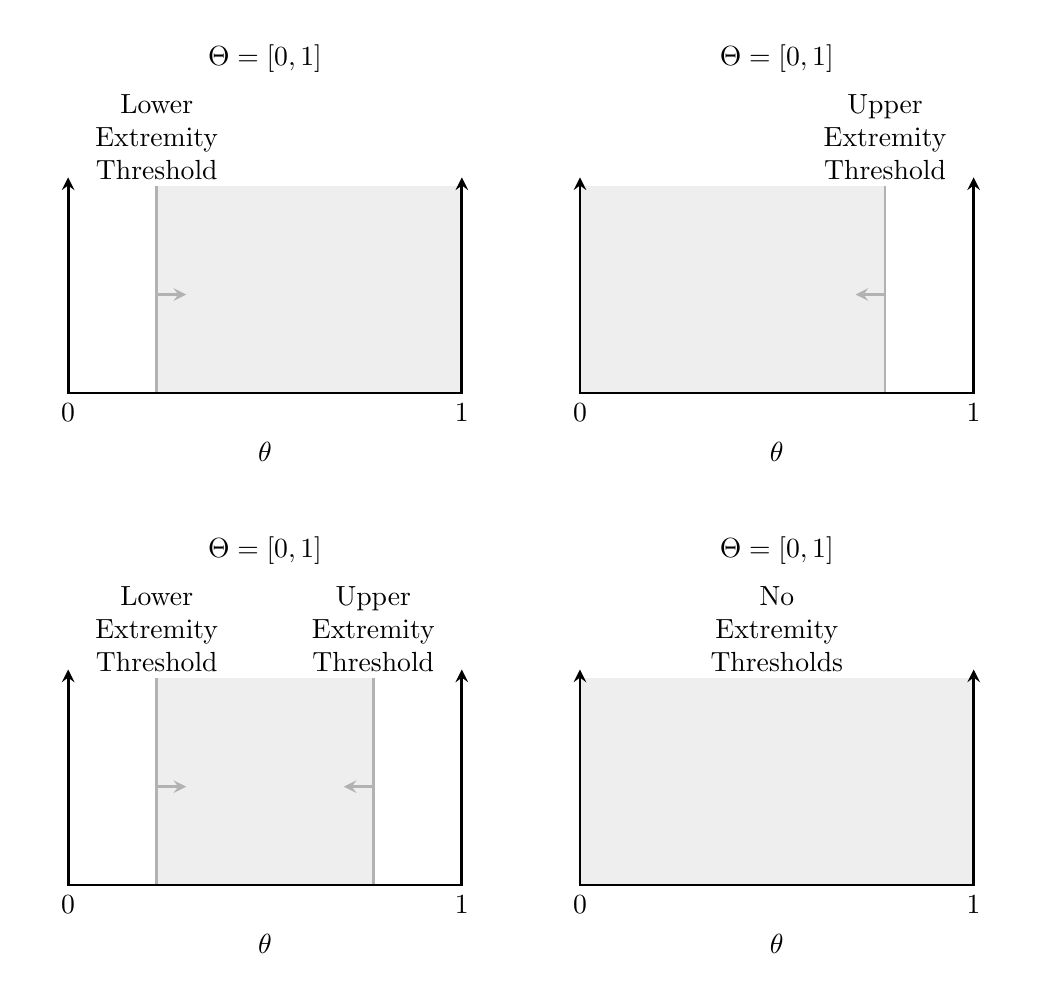
\begin{tikzpicture}[scale=0.25, thick]

  \begin{scope}[shift={(0, 0)}]
    \draw[white] (-12, -4.5) rectangle (12, 18.5);
    
    \node at (0, 17) { $\Theta = [0, 1]$ };
  
    \node[align=center] at (-5.5, 13) { Lower\\Extremity\\Threshold };
  
    \fill[color=gray80, opacity=0.33] (-5.5, 0) rectangle (10, 10.5);
    
    \draw[-, color=gray70, line width=1] (-5.5, 0) -- (-5.5, 10.5);
    \draw[->, >=stealth, line width=1, color=gray70] (-5.5, 5) -- +(1.5, 0);
  
    \draw[->, >=stealth, line width=1] (-10, -0.05) -- +(0, 11);
    \draw[->, >=stealth, line width=1] (+10, -0.05) -- +(0, 11);
    \draw[-, >=stealth, line width=1] (-10.05, 0) -- +(20.1, 0);
    
    \node[] at (-10, -1) { $0$ };
    \node[] at (+10, -1) { $1$ };
    
    \node[] at (0, -3) { $\theta$ };
    
  \end{scope}
  
  \begin{scope}[shift={(26, 0)}]
    \draw[white] (-12, -4.5) rectangle (12, 18.5);
    
    \node at (0, 17) { $\Theta = [0, 1]$ };
  
    \node[align=center] at (+5.5, 13) { Upper\\Extremity\\Threshold };
  
    \fill[color=gray80, opacity=0.33] (-10, 0) rectangle (5.5, 10.5);
  
    \draw[-, color=gray70, line width=1] (5.5, 0) -- (5.5, 10.5);
    \draw[->, >=stealth, line width=1, color=gray70] (5.5, 5) -- +(-1.5, 0);
  
    \draw[->, >=stealth, line width=1] (-10, -0.05) -- +(0, 11);
    \draw[->, >=stealth, line width=1] (+10, -0.05) -- +(0, 11);
    \draw[-, >=stealth, line width=1] (-10.05, 0) -- +(20.1, 0);
    
    \node[] at (-10, -1) { $0$ };
    \node[] at (+10, -1) { $1$ };
    
    \node[] at (0, -3) { $\theta$ };
    
  \end{scope}
  
  
  \begin{scope}[shift={(0, -25)}]
    \draw[white] (-12, -4.5) rectangle (12, 18.5);
    
    \node at (0, 17) { $\Theta = [0, 1]$ };
  
    \node[align=center] at (-5.5, 13) { Lower\\Extremity\\Threshold };
    \node[align=center] at (+5.5, 13) { Upper\\Extremity\\Threshold };
  
    \fill[color=gray80, opacity=0.33] (-5.5, 0) rectangle (5.5, 10.5);
    
    \draw[-, color=gray70, line width=1] (-5.5, 0) -- (-5.5, 10.5);
    \draw[->, >=stealth, line width=1, color=gray70] (-5.5, 5) -- +(1.5, 0);
  
    \draw[-, color=gray70, line width=1] (5.5, 0) -- (5.5, 10.5);
    \draw[->, >=stealth, line width=1, color=gray70] (5.5, 5) -- +(-1.5, 0);
  
    \draw[->, >=stealth, line width=1] (-10, -0.05) -- +(0, 11);
    \draw[->, >=stealth, line width=1] (+10, -0.05) -- +(0, 11);
    \draw[-, >=stealth, line width=1] (-10.05, 0) -- +(20.1, 0);
    
    \node[] at (-10, -1) { $0$ };
    \node[] at (+10, -1) { $1$ };
    
    \node[] at (0, -3) { $\theta$ };
    
  \end{scope}
  
  \begin{scope}[shift={(26, -25)}]
    \draw[white] (-12, -4.5) rectangle (12, 18.5);
    
    \node at (0, 17) { $\Theta = [0, 1]$ };
  
    \node[align=center] at (0, 13) { No\\Extremity\\Thresholds };
  
    \fill[color=gray80, opacity=0.33] (-10, 0) rectangle (10, 10.5);
  
    \draw[->, >=stealth, line width=1] (-10, -0.05) -- +(0, 11);
    \draw[->, >=stealth, line width=1] (+10, -0.05) -- +(0, 11);
    \draw[-, >=stealth, line width=1] (-10.05, 0) -- +(20.1, 0);
    
    \node[] at (-10, -1) { $0$ };
    \node[] at (+10, -1) { $1$ };
    
    \node[] at (0, -3) { $\theta$ };
    
  \end{scope}
  
\end{tikzpicture}

\end{document}  